\section{Question 2}
\paragraph{}
Consider the following potential

$$
	V(\phi) = \frac{\lambda}{4}(\phi^2 - v^2)^2
$$

where $\lambda > 0$ and $v > 0$. Plot this potential, and show that the minima of this potential is at $\phi_{min}=\pm v$.

\begin{figure}[H]
    \centering
    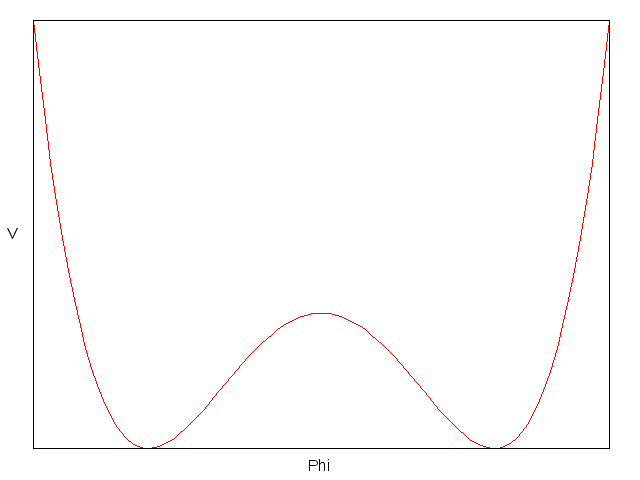
\includegraphics[width=0.5\textwidth]{q2-potential.png}
    \caption{Potential}
    \label{fig:q2-potential}
\end{figure}
%
\paragraph{}
Turning points of a function may be found when the first derivative of the function is equal to zero.

$$
	\frac{\partial V(\phi) } {\partial \phi}
	= \frac{\lambda}{4} 2 (\phi^2 - v^{2}) \times 2 \phi
	= \lambda (\phi^2 - v^{2}) \phi
$$

It can be seen that when this derivative is equal to zero that there are three possible solutions at $\phi=0$ and $\phi=\pm v^{2}$.  In order to identify which points are minima it is necessary to evaluate the second derivative of the potential at each of these points.

$$
	\frac{\partial ^2 V(\phi) } {\partial \phi ^2}
	= \lambda (\phi^{2} - v^{2}) + 2 \lambda \phi
$$

Evaluating the second derivateive at these points shows that the minima of this function are at $\phi=\pm v^{2}$ and that there is a maximum at $\phi=0$.


\paragraph{}
Considering the static solutions, where $\dot{\phi} = \ddot{\phi} = 0$. The Klein-Gordon Equation in this limit is then

$$
	\frac{\partial ^2 \phi } {\partial x^2} - \lambda (\phi ^{2} - v^{2})\phi = 0
$$